% Manuscript for Chaos: An Interdisciplinary Journal of Nonlinear Science
% (AIP), REVTeX 4.2 with the AIP `cha` journal option.
\documentclass[aip,cha,amsmath,amssymb,reprint]{revtex4-2}

\usepackage{graphicx}
\usepackage{booktabs}
\usepackage{xcolor}
\usepackage{hyperref}
\hypersetup{colorlinks=true, linkcolor=blue, citecolor=blue, urlcolor=blue}

\newcommand{\rtwo}{$R^2$}

\begin{document}

\title{Reading the rule beats learning it: interpretable estimators dominate deep
networks for the finite-horizon damage response of cellular automata}

% NOTE: placeholder (dummy) authors --- replace before submission.
\author{First A. Author}
\affiliation{Department of Data Analysis and Mathematical Modelling,
Example University, Example City, Country}
\author{Second B. Author}
\affiliation{Department of Data Analysis and Mathematical Modelling,
Example University, Example City, Country}

\date{\today}

\begin{abstract}
The behaviour of a cellular automaton (CA) is often summarised by
perturbation-defined statistics such as \emph{damage spreading}: evolve two
copies of a configuration that differ in one cell and watch the difference grow.
Because these statistics require running the simulator twice, estimating them
from a single observed space--time diagram is a natural task for a learned
amortiser---and a natural place to ask whether deep representation learning beats
transparent alternatives. We answer this with a pre-registered benchmark over the
elementary rule space and an enlarged two-state, radius-two space of $2^{32}$
rules, under an explicit observation protocol and leave-rules-out evaluation, and
we compare three estimators of four finite-horizon damage-response statistics: a
\emph{mechanistic} estimator that reads the local rule off the diagram and
simulates it; a regressor on five cheap single-diagram statistics; and an
anti-shortcut convolutional amortiser. The mechanistic estimator reaches the
Monte-Carlo reliability ceiling (median held-out \rtwo{} $0.99$) and
\emph{dominates} both the cheap statistics ($0.93$/$0.85$) and the deep network
($0.85$/$0.86$), everywhere. We explain why---the local rule is fully readable
from one diagram (recovered exactly; also decodable at $0.88$--$0.95$ from the
network's own bottleneck)---and quantify the deep model honestly: its only
measurable edge over five numbers is a modest increment on damage survival, the
least texture-like statistic, and it never nears the ceiling nor resolves
behaviour more finely in space. We turn the result into two constructive
outputs---a training-free, interpretable phenotype map for non-uniform CA, and a
data-driven map of where complex behaviour lives in rule space---and validate the
latter against an independent glider criterion. The recommendation for this task
is direct: read the rule.
\end{abstract}

\maketitle

\section{Introduction}
\label{sec:intro}

Cellular automata (CA) are the canonical minimal model of emergent
computation: a single local update rule, iterated in parallel, produces the full
zoo of behaviours from frozen order to chaos to the localized, interacting
``particles'' of complex, glider-supporting rules~\cite{wolfram2002,langton1990}.
Classifying that behaviour is a long-standing and subtle problem, because the
field distinguishes the \emph{genotype}---the local update rule---from the
\emph{phenotype}---the mesoscopic structure of the space--time diagram it
generates. A method that reads behaviour off the diagram must be prevented from
instead reading the \emph{rule} off the diagram, which is almost always possible:
a diagram contains, in its local neighbourhoods, the entire rule table, and a
convolutional network recovers the elementary rule with $99.9\%$ accuracy unless
architecturally stopped~\cite{rollier2024cnn}. This is a textbook instance of
\emph{shortcut learning}---deep vision models latch onto the most accessible
predictive cue rather than the intended one~\cite{geirhos2020shortcut}.

Compounding the difficulty, ``the behaviour class of a rule'' is not a single
well-defined quantity. Formalized Wolfram-style class membership is
undecidable~\cite{culikyu1988}, and the class observed in practice depends on the
initial-condition measure~\cite{gilman1987}, the lattice, and the observation
horizon. The defensible object is therefore not the rule but a \emph{protocol
tuple}---(rule orbit, IC measure, lattice, horizon)---characterized by
finite-horizon, perturbation-defined statistics. The best-posed of these is
\emph{damage spreading}: evolve two copies of a configuration that differ in a
single cell and measure how the difference grows~\cite{vispoel2024damage,
vispoel2022progress}. We are careful to call the resulting quantities
\emph{damage-response statistics}, not invariants: they are finite-size,
finite-horizon, and measure-dependent by construction.

Damage-response statistics stratify behaviour as theory predicts (dying damage
for order, ballistic space-filling for chaos, sub-ballistic sparse cones for
gliders) and, crucially, are defined through \emph{two} runs of the
simulator---so they are not a function of any single observed diagram. That last
property makes them a natural target for \emph{amortization}: train an encoder to
predict, from one diagram, a quantity that ordinarily requires a perturbation
experiment. If it succeeds and generalizes to unseen rules, one is tempted to
conclude the encoder has learned to read behaviour. But there is a transparent
alternative the deep model must beat: because the rule is readable, one can simply
\emph{infer the rule from the diagram and simulate the statistic}---an
interpretable, parameter-free estimator. Whether a learned representation
\emph{adds value} over this mechanistic estimator, or even over five cheap
statistics, is an empirical question, and exactly the kind that invites optimistic
framing after the fact. We therefore \emph{pre-registered} it.

This paper reports the benchmark. Under a fixed observation protocol, across the
elementary rule space and an enlarged two-state radius-two space of $2^{32}$
rules, we compare three estimators of the four damage-response statistics with
leave-rules-out evaluation and thresholds fixed in advance. The result is a
three-tier ordering that is the same everywhere we look: the mechanistic
rule-inference estimator reaches the Monte-Carlo reliability ceiling and
\emph{dominates}; five cheap single-diagram statistics capture most of the
signal through texture; and the deep amortiser, even built to resist the
rule-reading shortcut, never beats the cheap statistics overall and falls far
short of the ceiling. We prove the mechanism (the rule is fully recoverable from
one diagram, and pervades the network's own representation), bound the deep
model's one honest advantage (a modest increment on damage survival, the least
texture-like statistic), and turn the negative into two constructive outputs.

\section{Methods}
\label{sec:methods}

\subsection{Rule spaces and the observation protocol}
We use two rule spaces. \emph{Elementary CA} (ECA): two states, radius one, a
three-cell neighbourhood, $2^{2^3}=256$ rules, of which $88$ are distinct
representatives under the reflection and complementation symmetries a behavioural
method should respect. \emph{Radius-two CA}: two states, a five-cell
neighbourhood, a $32$-entry table and $2^{32}\approx4\times10^{9}$ rules; ECA is
the special case whose table ignores the two outer neighbours, so an embedded ECA
reproduces its elementary diagrams bit-for-bit (a continuity control). Because
the space is astronomically large we \emph{sample} it uniformly ($800$ rules) and
deduplicate by the order-four reflect/complement orbit.

Every quantity below is indexed by a fixed \emph{observation protocol}: a
Bernoulli$(1/2)$ initial condition on a ring of $127$ cells with periodic
boundaries, evolved from $t=0$. We avoid power-of-two widths, under which
additive rules collapse to homogeneity on a periodic ring and diverge from the
infinite-lattice reference behaviour. The horizon is capped so that the light cone
of a single perturbed cell cannot wrap the ring: $\lfloor w/(2r)\rfloor-1$ steps
for width $w$ and radius $r$, which for ECA is the familiar $\lfloor
w/2\rfloor-1$. These are deliberately short observations, and we return to their
scope in Sec.~\ref{sec:discussion}.

\subsection{Damage-response statistics}
The targets are four label-free scalars per rule, estimated from twin runs: draw
an initial condition, flip one cell, evolve both copies to the horizon, and
compare. \emph{Damage survival} is the probability that any difference remains;
conditional on survival, \emph{damage fraction} is the fraction of the ring that
differs, \emph{spreading rate} is the cone extent normalised by $2r$ times the
number of steps (so $1$ is light speed for any radius), and \emph{cone fill} is
the density of differing cells within the cone (high for chaos, low for sparse
gliders). Each vector is a Monte-Carlo average over $n_{\mathrm{pairs}}=256$
initial conditions; the per-rule random stream is keyed on the rule's identity, so
a rule's target is a well-defined function of $(\text{rule},\text{protocol})$,
independent of which other rules are computed alongside it
(Appendix~\ref{app:repro}).

\emph{Reliability ceiling.} Because each target is a single Monte-Carlo estimate,
no predictor can exceed its reliability. We draw $K=20$ independent replicates per
rule and fit a one-way random-effects model to get, per target, the intraclass
correlation ICC$(1)=\sigma^2_a/(\sigma^2_a+\sigma^2_e)$---the achievable-\rtwo{}
ceiling. On ECA the ceilings are $0.994$ (survival), $0.999$ (fraction), $0.9995$
(rate), $0.999$ (fill); on radius two, $0.987$/$0.998$/$0.998$/$0.980$. Survival
is the noisiest statistic (MC-noise std $0.022$) and, as we shall see, the one on
which the learned model has anything to add. Every \rtwo{} below is read against
these ceilings, not against $1$.

\subsection{Three estimators}
All three are trained on the same rules and evaluated with the \emph{same}
leave-rules-out split against the \emph{same} targets.

\emph{(i) Mechanistic rule-inference estimator.} We invert the forward map: from
one diagram we tabulate every observed neighbourhood$\to$next-cell transition and
rebuild the $2^{2r+1}$-bit rule table (entries never exercised default to $0$;
the observed \emph{coverage} is reported), then simulate the four statistics under
the identical protocol with an \emph{independent} random stream. When inference is
exact the estimate is simply a second independent Monte-Carlo draw of the target,
so its agreement with the cache is bounded by the reliability ceiling, not by any
learned capacity. The estimator has no trained parameters.

\emph{(ii) Five cheap statistics.} A regressor on five label-free single-diagram
features: the polarity-folded live-cell density, the temporal activity (fraction
of cells that change between rows), the zlib compression ratio, the $2\times2$
block entropy, and a radius-aware input-entropy variance (Wuensche's automated
glider screen~\cite{wuensche1999}). All five are (exactly or approximately)
invariant under the orbit symmetries. We report both a ridge and a
gradient-boosted-tree fit and take the stronger as the baseline of record.

\emph{(iii) Deep amortiser.} A convolutional network designed against the
rule-reading shortcut: $2\times2$ first-layer kernels (too small to span a
neighbourhood and its output together) feeding a signed $64$-dimensional
bottleneck and a linear head; a \texttt{predict\_map} variant emits a per-patch
map. It uses BatchNorm rather than GroupNorm in the regression encoder, which
keeps the per-patch map local. Training is $60$ epochs at $127$\,px; five seeds
vary weight initialization and minibatch order with the split and targets fixed.
The comparison is deliberately asymmetric in the network's favour: it has orders
of magnitude more parameters than a five-feature regressor. We stress that ``anti
shortcut'' names an architectural intent, not an achieved invariance---we measure
below that the rule remains fully recoverable from the network's representation,
which is precisely why the intent does not help.

\subsection{Statistics and pre-registration}
Every criterion, threshold, rule panel and control was committed to a timestamped
repository \emph{before} the corresponding measurement, and no threshold was
edited after a number was seen; the repository is released on publication so the
ordering is independently auditable. We report results \emph{per target}, never as
a four-target median alone, with the held-out \emph{rule} as the unit of
resampling. For each method pair we compute the paired difference in \rtwo{} with
a rule-level cluster bootstrap ($10^4$ resamples) and classify it by a
pre-registered rule: \emph{superiority} if the median $\Delta R^2\ge0.10$ and the
$95\%$ CI excludes $0$; \emph{practical equivalence} (TOST) if the $90\%$ CI lies
within $(-\delta,+\delta)$, $\delta=0.05$; otherwise inconclusive. A cross-fitted
\emph{stacking} test asks whether one method's prediction adds incremental \rtwo{}
beyond another's (margin $0.02$). Two descriptive claims are validated
independently: rule recoverability by linear probes on the network's bottleneck
versus the raw diagram and the five statistics; and the complex-rule landscape by
a localized-seed glider detector distinct from the damage signature.

\section{Results}
\label{sec:results}

\subsection{Three tiers, one ordering}
\label{sec:tiers}
Table~\ref{tab:tiers} is the paper in one place. Reading the rule and simulating
it recovers the damage-response statistics at the reliability ceiling and
\emph{dominates} both the cheap statistics and the deep amortiser, on the
elementary space, on the enlarged space, and on the held-out complex rules that
the enlarged space makes plentiful. The deep network never clears the
pre-registered advantage margin over five cheap statistics: it is beaten outright
on the elementary space and ties on the enlarged space and on complex rules
(Sec.~\ref{sec:paired}).

\begin{table*}[t]
\centering
\begin{ruledtabular}
\begin{tabular}{lcccc}
task & mechanistic & 5 statistics & deep CNN & ceiling \\
\colrule
ECA global & \textbf{0.999} & 0.927 & $0.852\pm0.015$ & 0.999 \\
radius-2 global & \textbf{0.991} & 0.845 & $0.864\pm0.014$ & 0.993 \\
radius-2 complex & \textbf{0.982} & 0.795 & $0.832\pm0.022$ & $\approx0.98$ \\
\end{tabular}
\end{ruledtabular}
\caption{Median leave-rules-out \rtwo{} of the three estimators against the
reliability ceiling. The interpretable mechanistic estimator sits at the ceiling
and dominates; the deep amortiser (mean\,$\pm$\,s.d.\ over five seeds; the other
methods are deterministic given the split) never beats five cheap statistics.}
\label{tab:tiers}
\end{table*}

The gap is starkest on \emph{damage survival}, the noisiest and least
texture-like statistic (Table~\ref{tab:eca}). There the mechanistic estimator
scores $0.985$ against a ceiling of $0.994$, while the five statistics reach only
$0.71$ and the CNN $0.67$---both leaving roughly a third of the achievable
variance on the table. On the texture-dominated statistics (fraction, rate, fill)
the cheap features already come close to the ceiling, and the deep model adds
nothing.

\begin{table*}[t]
\centering
\begin{ruledtabular}
\begin{tabular}{lcccc}
ECA target & mechanistic & 5 statistics & deep CNN & ceiling \\
\colrule
damage survival & 0.985 & 0.708 & 0.667 & 0.994 \\
damage fraction & 1.000 & 0.924 & 0.805 & 0.999 \\
spreading rate & 1.000 & 0.965 & 0.965 & 0.9995 \\
cone fill & 0.999 & 0.929 & 0.894 & 0.999 \\
\end{tabular}
\end{ruledtabular}
\caption{Per-target held-out \rtwo{} on the elementary space (deep CNN at the
reference seed). The mechanistic estimator is at the ceiling on every statistic;
the shortfall of the cheap features and the deep model is concentrated on
\emph{damage survival}.}
\label{tab:eca}
\end{table*}

\subsection{Paired inference: dominance and equivalence}
\label{sec:paired}
On the radius-two space (160 held-out rules, powered) the paired cluster bootstrap
confirms the ordering per target. The mechanistic estimator is
\emph{superior} to the cheap statistics on survival ($\Delta R^2=+0.17$), rate
($+0.12$) and cone fill ($+0.39$), and to the deep network on fraction, rate and
fill, with the remaining differences positive and excluding $0$. The deep network
and the cheap statistics, by contrast, \emph{trade}: the network is marginally
ahead on survival ($+0.08$) and the cheap features clearly ahead on cone fill
($-0.21$, baseline superior), with the rest a wash---neither dominates, and both
sit far below the mechanistic estimator. On the elementary space the held-out set
($18$ rules) is too small for tight per-target intervals; there we report the
median level of Table~\ref{tab:tiers}, where the cheap statistics beat the deep
network outright.

\subsection{Does the network add anything? A stacking test}
\label{sec:stacking}
The rigorous form of ``adds value'' is incremental: does a method's prediction
explain held-out residual variance beyond another's, under cross-fitting? The
answer is honest and specific (Table~\ref{tab:stacking}). Augmenting the five
statistics with the CNN's predictions yields a real, significant increment on
\emph{damage survival} ($+0.32$) and small increments on fraction and rate, but
none on cone fill; augmenting the CNN with the five statistics yields nothing.
The deep representation therefore does carry information the cheap features
miss---concentrated on survival, exactly the least texture-like statistic---but it
is dwarfed by the mechanistic estimator, whose increment over the five statistics
is $+0.14$ to $+0.84$ across targets. The learned model is not useless; it is
dominated.

\begin{table*}[t]
\centering
\begin{ruledtabular}
\begin{tabular}{lccc}
target & CNN over 5 stats & 5 stats over CNN & mechanistic over 5 stats \\
\colrule
survival & \textbf{+0.32} & $-0.01$ & +0.42 \\
fraction & +0.03 & +0.01 & +0.14 \\
rate & +0.03 & +0.01 & +0.16 \\
cone fill & $+0.08$\,(n.s.) & +0.08\,(n.s.) & +0.84 \\
\end{tabular}
\end{ruledtabular}
\caption{Cross-fitted incremental \rtwo{} (radius-two held-out rules). The CNN
adds significant information beyond the five statistics only on damage survival;
the five statistics add nothing beyond the CNN; the mechanistic estimator adds
far more than either, everywhere.}
\label{tab:stacking}
\end{table*}

\subsection{Why: the rule is readable}
\label{sec:probes}
The mechanism is that the local rule is fully present in one diagram. The
mechanistic inverter recovers it \emph{exactly} for $100\%$ of elementary rules
and $97.5\%$ of sampled radius-two rules (the remainder have under-covered tables,
the estimator's only failure mode, and the source of its sub-ceiling radius-two
score). The rule is not hidden from the network either: a linear probe reads the
rule's identity from the CNN's $64$-dimensional bottleneck at balanced accuracy
$0.88$ (ECA) and $0.95$ (radius two), and individual truth-table entries of unseen
rules at $0.78$/$0.61$---far above the five statistics' $0.69$/$0.55$ and the
majority baseline. The $2\times2$ ``anti-shortcut'' architecture thus does not
prevent rule recovery; the readable rule is the reason the deep model has nothing
to add that reading-and-simulating does not already provide.

\subsection{Constructive outputs}
\label{sec:constructive}
The negative has a constructive shadow. First, because the statistics are locally
and cheaply predictable, one can build \emph{training-free, interpretable}
phenotype maps for non-uniform CA by sliding the hand-crafted regressor over the
diagram. We validate this against an \emph{independent} local ground truth---the
damage response measured by local perturbation \emph{in} the composed system, not
the assumed pure-rule invariant---and score each map by the spatial correlation of
its per-column spreading-rate profile with that ground truth. With the
hand-crafted window selected on a validation split (not per-pair oracle), the
learned map shows \emph{no significant} localisation advantage over the cheap
window (Spearman $0.67$ vs $0.61$; $\Delta=+0.05$, $95\%$ CI $[-0.002,+0.10]$)---a
tie. The interpretable map is GPU-free and needs no training set.

Second, the same statistics over a uniform sample yield a data-driven picture of
\emph{where} complex behaviour lives (Fig.~\ref{fig:landscape}). We report this
conservatively: $\approx7.8\%$ of radius-two rules (Wilson $95\%$ CI $[6.9,8.8]\%$,
$n=3000$) \emph{satisfy the pre-registered damage-signature criterion}, versus
$\approx2\%$ of the $88$ elementary orbits. On the elementary space the criterion
selects exactly $\{54,106,110\}$---and $\{54,110\}$ are the literature's canonical
class-IV rules, so where independent ground truth exists the signature is
correct. An independent localized-seed glider detector agrees with the damage
signature on $92\%$ of the elementary rules it applies to (false-positive $6\%$,
false-negative $2\%$, the one miss being rule $54$, whose ether front advances at
light speed). On radius two, where no literature ground truth exists, the two
observables agree only $47\%$ of the time---so we make no claim that the $7.8\%$
are validated gliders, only that they satisfy the damage-signature shape.
Single-observable glider detection is itself unreliable in the large space.

\begin{figure}[t]
\centering
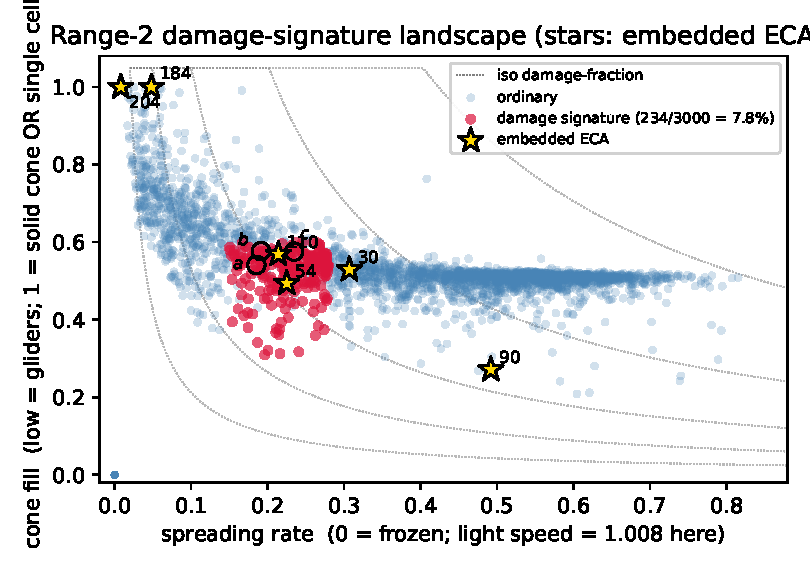
\includegraphics[width=\columnwidth]{figures/landscape.pdf}
\caption{The radius-two behaviour landscape from data ($n=3000$ uniformly sampled
canonical rules). Rules satisfying the pre-registered damage-signature criterion
(red)---persistent, sub-ballistic damage in a sparse cone---form a band between
the ordered arm and the chaotic bulk; the famous complex ECAs 54 and 110, embedded
into radius two, land in it (stars). The criterion is met by $\approx7.8\%$ of the
space versus $\approx2\%$ of the elementary orbits. On the elementary space the
criterion recovers exactly the literature class-IV set $\{54,110\}$ (plus the
borderline 106); on radius two it is a signature fraction, not an
independently validated glider count (Sec.~\ref{sec:constructive}).}
\label{fig:landscape}
\end{figure}

\section{Discussion}
\label{sec:discussion}

The benchmark returns the same answer three ways. For finite-horizon
damage-response statistics of cellular automata, an interpretable estimator that
reads the local rule and simulates it reaches the Monte-Carlo reliability ceiling
and dominates both a five-feature texture baseline and a deep amortiser---globally,
for held-out complex rules in a space where such rules are plentiful, and as a
spatial map. We read this as a \emph{structural} property of the task under the
tested protocol, not a failure of tuning, and we can say precisely why: the local
rule is fully readable from a single diagram (Sec.~\ref{sec:probes}), so any
statistic that is a smooth function of the rule is recoverable by whatever most
cheaply exposes it, and the exact route---reconstruct the generator and run
it---is available and interpretable.

We are careful not to overclaim the deep model's uselessness. The stacking test
(Sec.~\ref{sec:stacking}) shows the network does carry information beyond five
cheap statistics, concentrated on \emph{damage survival}---the least texture-like
of the four statistics, and the one whose reliability ceiling is lowest. This is
exactly where one would expect a learned representation to help: survival is a
rare-event probability that summary textures capture poorly. But the increment is
modest, it is confined to that one statistic, and it does not lift the network's
end-to-end predictions above the cheap baseline, let alone toward the ceiling that
the mechanistic estimator reaches. The honest reading is not ``deep learning adds
nothing'' but ``an interpretable estimator dominates, and the learned model's one
real edge---survival---is small and does not change the recommendation.''

\emph{Scope.} The claim is deliberately narrow: it concerns damage-response
statistics under one observation protocol (Bernoulli$(1/2)$ initialization, width
$127$, a horizon of $\sim\!62$ steps for ECA and $\sim\!30$ for radius two) on
two-state CA. These are short observations, and the statistics are, by
construction, protocol-dependent~\cite{gilman1987,culikyu1988}; a companion
sensitivity analysis confirms that the induced taxonomy shifts with the
IC measure and lattice, which is why we index every claim by the tuple rather than
by ``the rule.'' Statistics that depend on genuinely non-local or rare structure
that summary textures miss---long transients, specific particle interactions,
computational depth---might still reward a learned representation, and the survival
increment we measure is a small hint in that direction. Identifying a target and
regime where a learned representation beats reading-and-simulating is the natural
next step; the natural extension to a predictive, forecasting objective, however,
we expect to inherit the same shortcut, since forecasting future rows is trivial
once the rule is recovered.

Our result sits squarely in the shortcut-learning
literature~\cite{geirhos2020shortcut} and in the older recognition that no
unsupervised taxonomy is ``just there'' in data without a chosen
similarity~\cite{kleinberg2002}: here the cheapest similarity---texture---already
captures most of the signal, and the most faithful route---reading the
rule---captures all of it, so the deep model is squeezed from both sides. For the
task as usually posed, the recommendation is to read the rule and, where that is
undesirable, to compute the cheap features and skip the network.

\appendix
\section{Reproducibility}
\label{app:repro}

All experiments run on a single Apple-silicon machine (Metal/CPU, fp32); the
pipeline is first-party except for the gradient-boosted-tree and ridge baselines
(\texttt{scikit-learn}) and PyTorch. The amortiser error bars come from five
training seeds that vary only weight initialization and minibatch order; the
leave-rules-out split, the diagram cache and the targets are keyed on their own
fixed seeds, so the spread measures optimisation-seed variance alone. The
mechanistic estimator and the reliability ceiling are deterministic given the
protocol.

\emph{Target well-definedness.} Each rule's damage-response target is estimated
from an initial-condition stream seeded on the rule's identity, so the value is
independent of which other rules are computed alongside it. An earlier
implementation seeded the stream by the rule's position in the sorted panel; we
measured the resulting cross-panel drift at up to $0.05$--$0.08$ on
borderline-survival rules (unbiased Monte-Carlo resampling, but panel-dependent)
and removed it, verifying zero drift under identity keying---the one deviation
from the original pre-registration, disclosed here. The intrinsic estimation noise
at $n_{\mathrm{pairs}}=256$ is quantified per target by the reliability analysis
(Sec.~\ref{sec:methods}).

The complete pre-registered criteria, the training and evaluation code, the
sampled rule panels, and the cached targets will be released under the MIT license
upon publication.

\bibliographystyle{apsrev4-2}
\bibliography{refs}

\end{document}
